% !TEX encoding = UTF-8
% !TEX program = pdflatex
% !TEX root = InformationRetrieval.tex
% !TEX spellcheck = it-IT

% 28 Ottobre 2016
\subsubsection{Maximum Likelihood}

Per trovare il valore di $p$ che più si avvicina alla sequenza di osservazioni è necessario effettuare la derivata della formula precedente e porla uguale a 0. Questo calcolo è complesso e quindi si preferisce effettuare la derivata del logaritmo.
Ad esempio se la sequenza di osservazioni del lancio di una moneta è $T,T, C$, se provo a tracciare un grafico della funzione in base al variare di $p$ ho un massimo con $p = 2/3$, che coincide con la probabilità che ho osservato di ottenere testa.

Assumiamo quindi di avere $D = \{x, \overline{x}, x, x, \ldots \}$, dove $x$ è un documento che contiene una determinata parola e $\overline{x}$ è un documento che non la contiene.
Si ha che la probabilità $P(D|\rel)$ prende il nome di \textbf{likelihood} e che l'operazione di massimizzazione di questa probabilità prende il nome di \textbf{maximum likelihood}.

Da notare che $P(D|\rel)$ è un'abbreviazione per $P(W = x, W = \overline{x}, W = x \ldots | C = \rel)$.

\begin{align*}
	&\frac{\partial}{\partial p} \log \Big( (D|\rel) \Big) = 0\\
	&\frac{\partial}{\partial p} \log \Big( \prod\limits_{j = 1}^n p^{x_j}(1-p)^{1-x_j} \Big) = 0\\
	&\frac{\partial}{\partial p} \sum\limits_{j = 1}^n \log \Big( p^{x_j}(1-p)^{1-x_j} \Big) = 0 \\
	&\frac{\partial}{\partial p} \sum\limits_{j = 1}^n \log \Big( p^{x_j}\Big) + \sum\limits_{j = 1}^n \log \Big((1-p)^{1-x_j} \Big) = 0 \\
	&\frac{\partial}{\partial p} \sum\limits_{j = 1}^n x_j \log \Big( p\Big) + \sum\limits_{j = 1}^n (1-x_j)\log \Big(1-p \Big) = 0 \\
	&\frac{1}{p}\sum\limits_{j = 1}^n x_j + \sum\limits_{j = 1}^n (1-x_j) \frac{1}{1-p}(-1)= 0 \\
	&\frac{n_{tR}}{p}  =  \frac{N_R}{1-p} - \frac{N_{tR}}{1-p}\\
	&(1-p)n_{tR} = (N_r - n_{tR}) p  = N_Rp - n_{tR}p\\
	&\boxed{p = \frac{n_{tR}}{N_R}}
\end{align*}

\noindent dove:
\begin{itemize}
	\item $N_{tR} = \sum\limits_{j = 1}^n x_j$ è il numero di volte che ho osservato il termine $x$ tra i documenti rilevanti.
	\item $N_R = \sum\limits_{j = 1}^n 1$ è il numero di documenti rilevanti.
\end{itemize}

\begin{figure}[htbp]
	\centering
	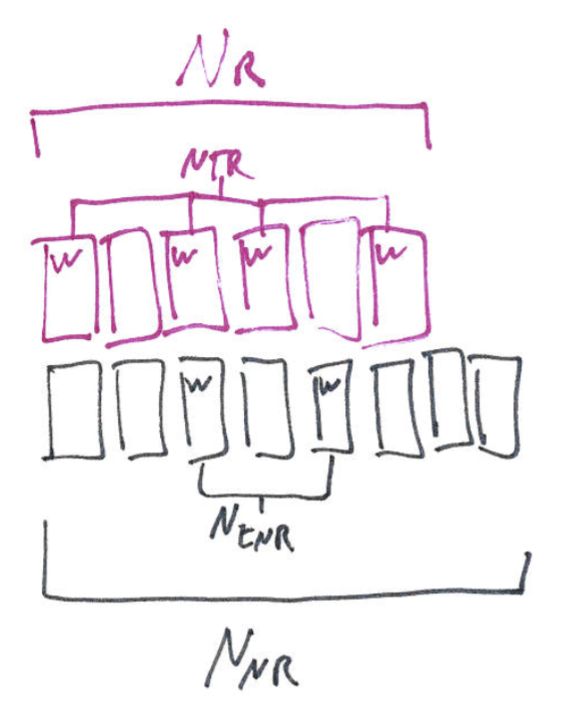
\includegraphics[width=.35\textwidth]{images/l10-fig-1}
	\caption{$N_R, N_{tR}, N_{NR}$ e $N_{tNR}$}
\end{figure}

Gli stessi conti possono essere ripetuti per calcolare $q$, ottenendo:

$$
\boxed{q = \frac{n_{tNR}}{N_{NR}}}
$$

\noindent Dove $N_{tNR}$ è il numero di volte che ho osservato il termine $x$ tra i documenti non rilevanti e $N_{NR}$ è il numero di documenti non rilevanti.

Si ha quindi che 

$$
N = N_R + N_{NR} \qquad \text{e} \qquad n_t = n_{tR} + n_{tNR}
$$

e che $q$ può essere espresso come:

$$
q = \frac{N_t - N_{tR}}{N - N_r}
$$

Un documento viene quindi classificato come rilevante quando

\begin{align*}
	P(C = \rel | X) &> P(C = \notrel | X)\\
	P(X | C=\rel)P(C=\rel) &> P(C = \notrel |X)P(C = \notrel) \\
	\Big( \frac{p}{1-p} \Big)^x(1-p) P(C = \rel) &> \Big(\frac{q}{1-q}\Big)^x (1-a)P(C = \notrel)
\end{align*}

Il tutto sotto l'ipotesi di una \textbf{zero-one loss function}, ovvero nel caso in cui effettuare un errore di classificazione abbia lo stesso peso per entrambe le classi.

Tutto questo vale però se abbiamo solo una moneta (o parola).

\paragraph{Smoothing delle probabilità} C'è un problema se $N_{tR} = 0$, perché il questo caso si ha che $P(C = \rel | D) = 0$. Ovvero, se non ci sono documenti rilevanti con quel termine, la probabilità che un documento con quel termine diventa 0, ma può essere che $N_{tR}$ sia 0 perché non sono ancora stati osservati documenti con rilevanti contenenti quel termine e non perché il termine non è significativo per la rilevanza del documento.

La probabilità $p$ viene quindi calcolata con dei termini di smoothing:

$$
p = \frac{N_{tR} + \alpha}{N_R + \alpha + \beta}
$$

Ci sono alcune configurazioni notevoli dei termini:

\begin{itemize}
	\item \textbf{Laplace's Smoothing}: $\alpha = \beta = 1$
	\item \textbf{Jeffrey's Smoothing}: $\alpha = \beta = 0.5$. Questi valori vengono utilizzati anche nel \textbf{Binary Indipendence Model} (\textbf{BIM}).
\end{itemize}


\subsubsection{Caso con più variabili}

$$
P(C = \rel | D=(T_1, T_2, T_3)) = \frac{P(D=(T_1,T_2, T_3) | C=\rel)P(C=\rel)}{P(D=(T_1, T_2, T_3))}
$$

\noindent In questo caso l'esperimento consiste nel lancio in contemporanea di 3 monete, o nel caso della rilevanza dei documenti, la presenza o meno di più termini.
Continuano inoltre a valere le ipotesi delle variabili i.i.d.

Possiamo quindi calcolare $P(D=(T_1,T_2, T_3) | C=\rel)$ con

$$
P(D=(T_1,T_2, T_3) | C=\rel) = \prod\limits_{j=1}^{n} P((T_1, T_2,T_3)_j | C = \rel)
$$

Dove $(T_1, T_2,T_3)_j$ rappresenta il $j$-esimo documento, ad esempio: $(T_1 = t_1, T2 = \overline{t_2},T_3 = \overline{t_3})_3$ rappresenta il terzo documento, il quale contiene solo il termine $t_1$.

\begin{figure}[htbp]
	\centering
	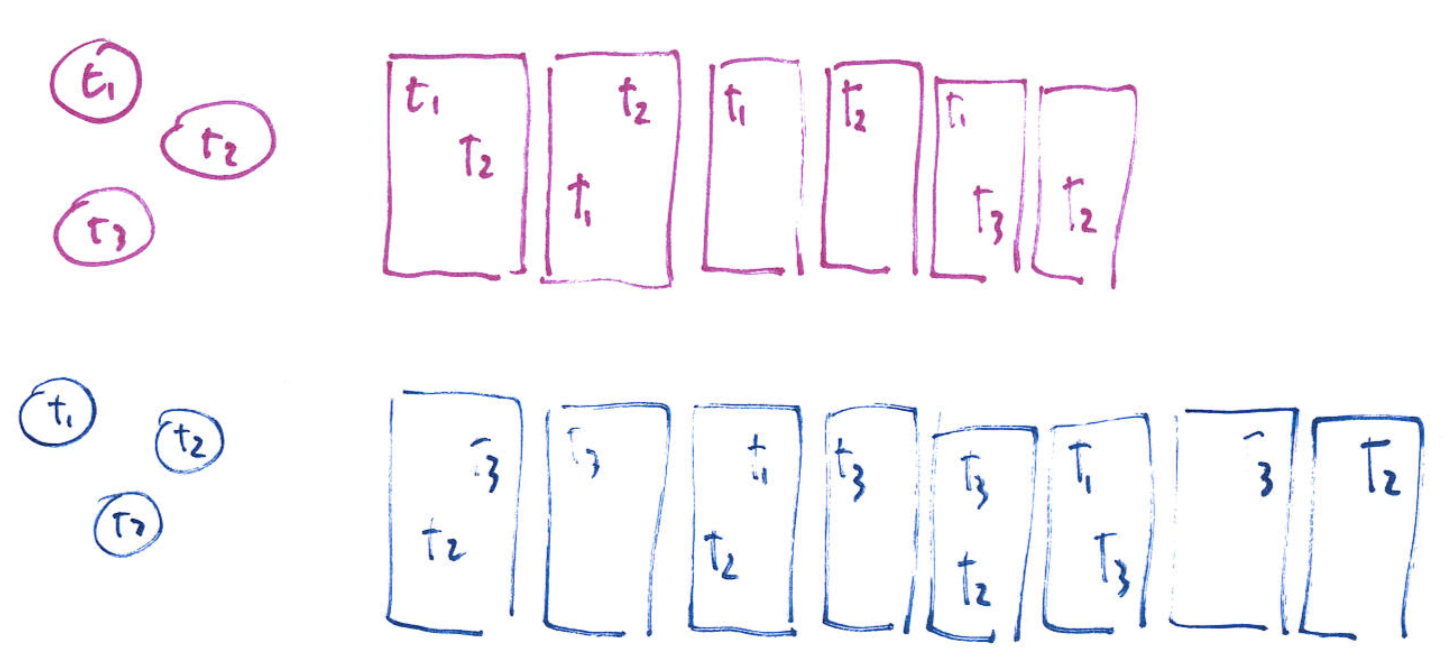
\includegraphics[width=.5\textwidth]{images/l10-fig-2}
	\caption{Rappresentazione grafica della collezione. In viola i documenti rilevanti, in blu quelli non rilevanti.}
\end{figure}

Anche in questo caso la probabilità $P((T_1, T_2,T_3)_j | C = \rel)$ può essere calcolata andando ad osservare quante volte compaiono le varia combinazioni di termini all'interno dei documenti.
Il problema è che per avere una stima decente della probabilità devo osservare minimo 8 esiti, perché altrimenti alcune combinazioni non potrebbero mai uscire.
Questo è un problema perché il numero minimo di esiti cresce in modo esponenziale rispetto al numero di termini/parole $2^{|V|}$(\textbf{curse dimensionality}).

Per gestire questo problema viene fatta un'assunzione d'indipendenza: la cosi detta \textbf{Naive Bayes Indipendence Assumption}.
Grazie a questa assunzione posso semplificare il calcolo in:

$$
P(C = \rel | D=(T_1, T_2, T_3)) = \prod\limits_{i = 1}^{|V|}P(T_i|C=\rel)
$$

\noindent dove $V$ è il vocabolario dei termini, $V = \{ T_1, T_2, \ldots T_m\}$.

Nel nostro caso abbiamo anche che

$$
P(T_i|C=\rel) \approx \text{Bernoulli}(p_i)
$$

\noindent perché possiamo dare ad ogni termine un certo peso.
Il problema adesso è quale peso dare ai vari termini.

Assumiamo che ci siano 4 documenti che sappiamo essere rilevanti e che contengono rispettivamente i termini $(t_1, t_3), (t_2), (t_1), (t_3)$. Abbiamo quindi:

\begin{align*}
P(D | C=\rel) &= \prod\limits_{j=1}^n P((T_{1},T_{2},\ldots T_{m})_j|C=\rel) \\
&= \prod\limits_{j=1}^n \prod\limits_{i=1}^m P((T_i)_j | C=\rel)
\end{align*}


\noindent Per calcolare le singole probabilità possiamo utilizzare le formule precedentemente viste:

$$
p_i = \frac{N_{t_iR}}{N_R} \qquad \text{e} \qquad q_i = \frac{N_{t_iNR}}{N_{NR}}
$$

\noindent Dove $N_{t_iR}$ indica il numero di documenti rilevanti contenenti il termine $t_i$. Anche in questo caso possono essere applicati dei termini di smoothing specifici per ogni termine.

Quindi, per sapere se un documento $D$ che contiene i termini $t_1$ e $t_3$ ma non $t_2$ è rilevante, possiamo utilizzare:

\begin{align*}
P(C=\rel | D=\{t_1, \overline{t_2}, t_3\}) &=\frac{ P( D=\{t_1, \overline{t_2}, t_3\} |C = \rel)P(C=\rel)}{P( D=\{t_1, \overline{t_2}, t_3\})} \\
                                           &=\frac{\prod\limits_{i=i}^{|V|} P(T_i | \rel)P(\rel) }{P( D=\{t_1, \overline{t_2}, t_3\})} \\
                                           &=\frac{\prod\limits_{i=i}^{|V|}p_{i}^{t_i}(1-p_i)^{1- t_i} }{P( D=\{t_1, \overline{t_2}, t_3\})}
\end{align*}

\noindent con le probabilità che possono o essere stimate o calcolate con le formule viste precedentemente. Lo stesso vale anche per $\notrel$.

Ma quando è che classifichiamo un documento come non rilevante? Quando

\begin{align*}
									                        P(C=\rel|D) &> P(C=\notrel |D) \\
									\frac{P(D | C=\rel)P(C=\rel)}{P(D)} &> \frac{P(D | C=\notrel)P(C=\notrel)}{P(D)} \\
									             P(D | C=\rel)P(C=\rel) &> P(D | C=\notrel)P(C=\notrel) \\
			\Bigg[\prod\limits_{i=1}^{|V|} p_{i}^{t_i} (1 - p_{i})^{(1-t_i)}\Bigg] P(C = \rel) &> \Bigg[\prod\limits_{i=1}^{|V|} q_{i}^{t_i} (1 - q_{i})^{(1-t_i)}\Bigg]P(\notrel) \\
  \Bigg[\prod\limits_{i=1}^{|V|} \bigg(\frac{ p_{i} }{1-p_i}\bigg)^{t_i} (1-p_i)\Bigg] P(rel) &>\Bigg[\prod\limits_{i=1}^{|V|} \bigg(\frac{ q_{i} }{1-q_i}\bigg)^{t_i} (1-q_i)\Bigg] P(\overline{rel})
\end{align*}

\noindent Se la disequazione è rispettata, allora il documento può essere classificato come rilevante.

C'è però un problema, perché nel caso pratico ci sono vocabolari da 100000 termini e quindi le produttorie risultano essere incalcolabili, perché i numeri diventano troppo piccoli.
Per raggiare questo problema è necessario prendere il logaritmo delle produttorie, in modo da poter riscriverle come sommatorie:

\begin{align*}
\log \Bigg(\Bigg[\prod\limits_{i=1}^{|V|} \bigg(\frac{ p_{i} }{1-p_i}\bigg)^{t_i} (1-p_i)\Bigg] P(rel)\Bigg) &>\log\Bigg(\Bigg[\prod\limits_{i=1}^{|V|} \bigg(\frac{ q_{i} }{1-q_i}\bigg)^{t_i} (1-q_i)\Bigg] P(\overline{rel})\Bigg) \\
\sum\limits_{i=1}^{|V|} \log\big( p_{i}^{t_i} (1 - p_{i})^{(1-t_i)} \big) P(\rel) &> \sum\limits_{i=1}^{|V|} \log\big( q_{i}^{t_i} (1 - q_{i})^{(1-t_i)} \big) P(\notrel) \\
\sum\limits_{i=1}^{|V|} \log\bigg( \frac{ p_{i} }{1-p_i} \bigg)^{t_i} +\sum\limits_{i=1}^{|V|} \log(1-p_i) + \log(P(\rel)) &> \ldots \\
\sum\limits_{i=1}^{|V|} t_i \log\bigg( \frac{ p_{i} }{1-p_i} \bigg) + \underbrace{\sum\limits_{i=1}^{|V|} \log(1-p_i) + \log(P(\rel))}_{\text{non dipende dal documento}} &> \sum\limits_{i=1}^{|V|} t_i \log\bigg( \frac{ q_{i} }{1-q_i} \bigg) +\underbrace{\sum\limits_{i=1}^{|V|} \log(1-q_i) + \log(P(\overline{rel}))}_{\text{non dipende dal documento}}
\end{align*}

\noindent Con questa nuova formulazione si ha che alcuni pezzi devono essere calcolati solo una volta ed inoltre se il termine $t_i$ non compare nel documento ($t_i=0$), non lo considero nella sommatoria e quindi nel lato pratico le sommatorie non vengono calcolate su tutto il dizionario, ma solo sui termini che compaiono nei documenti.

Posso inoltre riformulare ancora, portando tutte le sommatoria da una parte, ottenendo:

$$
\underbrace{\sum\limits_{i=1}^{|V|} t_i \log\bigg( \frac{p_i}{q_i} \frac{1-q_i}{1-p_i}\bigg)}_{\text{\textbf{dipende} dal documento}} + \underbrace{\sum\limits_{i=1}^{|V|} \log \bigg( \frac{1-p_i}{1-q_i} \bigg) + \log \frac{P(\rel)}{P(\notrel)}}_{\text{\textbf{non dipende} dal documento}} > 0
$$

\noindent Nella nuova riformulazione solo la parte sinistra dipende dal documento, mentre quella destra è costante per tutta la collezione.
Inoltre, il logaritmo della parte sinistra soffre delle stesso problema che si aveva nel caso in cui un termine non compare mai all'interno di un documento.
Quindi di solito si aggiungo delle costanti ($+0.5$) sia al numeratore che al denominatore, ottenendo così il \textbf{relevance weight} di un termine:

\begin{align*}
	relevance \ weight_i  &\approxeq \log\bigg( \frac{p_i(1-q_i)}{(1-p_i)q_i} \bigg)	 \\
						  &= \log\bigg( \frac{N_{t_iR} + 0.5}{N_R - N_{t_iR} + 0.5} \frac{N_{NR} - N_{t_{iNR}}+ 0.5}{N_{t_iNR}+ 0.5} \bigg)		        
\end{align*}

\noindent Così facendo quando non ho informazioni riguardanti i documenti rilevanti nel motore di ricerca o classificatore, ovvero $N_R = N_{t_iR} = 0 $, riesco comunque a fornire un peso per il termine. 

$$
relevance \ weight_i = \log\bigg( \frac{N_{NR} - N_{t_{iNR}}+ 0.5}{N_{t_iNR}+ 0.5} \bigg)
$$

\noindent Inoltre, così facendo ottengo una giustificazione probabilistica per \textbf{IDF}.

\begin{align*}
idf(t_i)				&=  \frac{N}{N_t} \\
\log\big(idf(t_i) \big) &= \log\big( \frac{N}{N_t}\big) 
\end{align*}

dato che $N_{t_{iNR}} \ll N_{NR}$, perché sono nell'ipotesi che non ci sono informazioni riguardo i documenti rilevanti ($N_{NR} = N$) e il numero di documenti in cui compare il termine $t_i$ è tipicamente molto minore del numero totale di documenti, ottengo:

\begin{align*}
w_i &=\log\bigg( \frac{N_{NR} - N_{t_{iNR}}+ 0.5}{N_{t_iNR}+ 0.5} \bigg) \\
    &\approxeq \log\bigg( \frac{N_{NR} + 0.5}{N_{t_iNR}+ 0.5} \bigg) \\
    &\approxeq log\big( \frac{N}{N_t}\big) = \log\big(idf(t_i) \big)
\end{align*}















